\documentclass{../Template}
\addbibresource{../Bibliografia.bib} % si quieres incluir la bibliografía

\RequirePackage{transparent}


% Define el campo de subtitle como variable
\newcommand{\subtitle}[1]{\gdef\@subtitle{#1}}

% Macro para hacer el título
\newcommand{\MakeTitle}[2]{%
  \begin{titlepage}
    \begin{tikzpicture}[remember picture, overlay]
      % Fondo de color (opcional)
      \fill[#1!50] (current page.south west) rectangle (current page.north east);


      % Texto centrado
      \node[align=center, text width=0.9\paperwidth] at (current page.center) {
        {\Huge\bfseries\color{white} \thetitle\par}
        \vspace{1em}

        {\LARGE\itshape\color{white} \@subtitle\par}
        \vspace{3em}

        {\Large\color{white} \theauthor\par}

        \vspace{4em}d
        {\large\color{white} \today}
      };
    \end{tikzpicture}
    \null % Para evitar espacios verticales no deseados
    \thispagestyle{empty}
    \clearpage
  \end{titlepage}
}

% Para que \title y \author funcionen con \thetitle y \theauthor
\pretitle{\gdef\thetitle}
\preauthor{\gdef\theauthor}




%----------------------------------------------------------------------------
% ÍNDICE PERSONALIZADO
%----------------------------------------------------------------------------

\addto\captionsspanish{\renewcommand{\contentsname}{Índice general}}
\let\oldtableofcontents\tableofcontents
\renewcommand{\tableofcontents}{\begingroup\oldtableofcontents\endgroup}

% Comandos para poder hacer la división en lineas -> Aun hay que modificar las líneas 
\newcommand{\hLinefill}[1]{\rule[0.5ex]{#1\linewidth}{0.4pt}}
\newcommand{\NewPart}[2]{
    \addtocontents{toc}{%
        \begingroup%
            \setlength{\parindent}{0pt}%
            \protect \Large\bfseries \hLinefill{#2} \hspace*{4mm} \ #1 \ \hspace*{4mm} \hLinefill{#2} \protect\par%
        \endgroup%
    }%
}

% Macro De Ejemplo

\newcounter{Ejemplo}[chapter]
\newcounter{Teorema}[chapter]
\newcounter{Definicion}[chapter]
\newcounter{Ejercicio}[chapter]

\colorlet{ColorEjemplo}{red!75!black}
\colorlet{ColorTeorema}{blue!75!black}
\colorlet{ColorDefinicion}{green!75!black}
\colorlet{ColorEjercicio}{gray!65!black}

\newtcolorbox[use counter=Ejemplo]{Ejemplo}[1]{%
empty,title={Ejemplo \thechapter.\thetcbcounter: #1},attach boxed title to top left,
boxed title style={empty,size=minimal,toprule=2pt,top=4pt,
overlay={\draw[ColorEjemplo,line width=2pt]
([yshift=-1pt]frame.north west)--([yshift=-1pt]frame.north east);}},
coltitle=ColorEjemplo,fonttitle=\large\bfseries,
before=\par\medskip\noindent,parbox=false,boxsep=0pt,left=0pt,right=3mm,top=4pt,
breakable,pad at break*=0mm,vfill before first,
overlay unbroken={\draw[ColorEjemplo,line width=1pt]
([yshift=-1pt]title.north east)--([xshift=-0.5pt,yshift=-1pt]title.north-|frame.east)
--([xshift=-0.5pt]frame.south east)--(frame.south west); },
overlay first={\draw[ColorEjemplo,line width=1pt]
([yshift=-1pt]title.north east)--([xshift=-0.5pt,yshift=-1pt]title.north-|frame.east)
--([xshift=-0.5pt]frame.south east); },
overlay middle={\draw[ColorEjemplo,line width=1pt] ([xshift=-0.5pt]frame.north east)
--([xshift=-0.5pt]frame.south east); },
overlay last={\draw[ColorEjemplo,line width=1pt] ([xshift=-0.5pt]frame.north east)
--([xshift=-0.5pt]frame.south east)--(frame.south west);},%
}


\newtcolorbox[use counter=Teorema]{Teorema}[1]{%
empty,title={Teorema \thechapter.\thetcbcounter: #1},attach boxed title to top left,
boxed title style={empty,size=minimal,toprule=2pt,top=4pt,
overlay={\draw[ColorTeorema,line width=2pt]
([yshift=-1pt]frame.north west)--([yshift=-1pt]frame.north east);}},
coltitle=ColorTeorema,fonttitle=\large\bfseries,
before=\par\medskip\noindent,parbox=false,boxsep=0pt,left=0pt,right=3mm,top=4pt,
breakable,pad at break*=0mm,vfill before first,
overlay unbroken={\draw[ColorTeorema,line width=1pt]
([yshift=-1pt]title.north east)--([xshift=-0.5pt,yshift=-1pt]title.north-|frame.east)
--([xshift=-0.5pt]frame.south east)--(frame.south west); },
overlay first={\draw[ColorTeorema,line width=1pt]
([yshift=-1pt]title.north east)--([xshift=-0.5pt,yshift=-1pt]title.north-|frame.east)
--([xshift=-0.5pt]frame.south east); },
overlay middle={\draw[ColorTeorema,line width=1pt] ([xshift=-0.5pt]frame.north east) 
--([xshift=-0.5pt]frame.south east); },
overlay last={\draw[ColorTeorema,line width=1pt] ([xshift=-0.5pt]frame.north east)
--([xshift=-0.5pt]frame.south east)--(frame.south west);},%
}


\newtcolorbox{Resaltar}{
  colback=Gray!40,    % Color de fondo
  colframe=Gray!40,   % Color del borde
  sharp corners,      % Esquinas cuadradas
  boxrule=0pt,        % Grosor del borde (0pt para que desaparezca)
  left=5pt,           % Margen izquierdo interno
  right=5pt,          % Margen derecho interno
  top=5pt,            % Margen superior interno
  bottom=5pt          % Margen inferior interno
}

% Definiciones del título
\title{Deep Learning}
\subtitle{Con aplicaciones en Python}
\author{Daniel Vázquez Lago}

% Documento

\begin{document}
\MakeTitle{1}{blue!80!black}{Snow1}


\setlength{\parskip}{2.2mm} % Cambia el espacio entre párrafos

\newpage

\tableofcontents


\NewPart{Redes Neuronales}{0.31}

\chapter{Introducción}
\chapter{Fundamentos del aprendizaje máquina}

\section{Clasficiación Binaria}

Para poder avanzar en el tema, primero tenemos que definir algunos de los términos que hemos usado de manera intuitiva: aprendizaje, experiencia, mejora y tarea. Empecemos con la tarea de la clasificación binaria. 

Supongamos un problema abstracto en el cual tenemos los datos de la siguiente forma: 

\begin{equation}
    D = \{ (x_1,y_1),(x_2,y_2),\ldots, (x_n,y_n) \}
\end{equation}
donde $x\in \mathbb{R}^n$ e $y=\pm 1$. A pesar de que $D$ represente todos los datos, nosotros solo tenemos acesso a un subconjunto de ellos, $S\in D$. Usando $S$, nuestra tarea será generar un proceso computacional que implemente la función $f:x\to y$  tal que podemos usar $f$ para predecir los datos no pertenecientes a $S$, esto es,  $x_i, y_i\notin S$, tal que $f(x_i)=y_i$. Si dennotamos  $U$ como el conjunto contario a $S$ ($U=\bar{S}$), podemos suponer que una medida de la eficiencia/calidad de nuestro sistema para realizar esta tarea vendrá dada por una función error sobre los datos no vistos: 

\begin{equation}
    E(f,D,U) = \frac{\sum_{x_i,y_i \in U} [f(x_i)\neq y_i] }{|U|}
\end{equation} 
Medimos el rendimiento de la tarea usando la función error $E(f,D,U)$ sobre los datos no conocidos $U$. EL tamaño de los datos conocidos $S$ será nuestra ``experiencia''. Lo que nosotros queremos hacer es crear algoritmos que generen funciones $f$ (comunmente denominadas modelos).  En general a los valores $x$ se le llaman valores de entradas o \textit{inputs}, mientras que a $y$ valores de salida o \textit{outputs}.

Como en cualquier otra disciplina, las características computacionales es un aspecto relevante, pero además de tener en cuenta los costos computacionales, tendremos que tratar de hallar el modelo $f$ que tenga el menor errror posible $E(f,D,S)$ con el menor $|S|$ posible. 

\begin{Ejemplo}{Web de Comercio Electrónico}
    Supongamos que queremos implementar en una página web una página personalizada para usuarios registrados, que les muestre los productos que más dispuestos estarían a comprar. La web registra la información de los usuarios. ¿Cómo se relaciona este problema con la clasificación binaria? 

    Esta claro que el problema relaciona productos con personas. Centremonos entonces en la relación entre un solo producto y un solo usuario. Lo que nosotros queremos saber es si va a ser comprado. Podemos denotar el estado ``deseado'' con $y=+1$ mientras que el estado ``no deseado'' por $y=-1$. Lo siguiente que debemos hacer es coger información del producto (tipo de producto...) y la información histórica de búsqueda y compra del usuario, representado todo esto en un vector $x \in \mathbb{R}^n$. Basados en esta información y en el mapeo conocido $\{(x_1,y_1),(x_2,y_2),\ldots,(x_n,y_n)\}$, entonces podemos generar la función modelo $f:x\to y$ a partir lo cual podemos determinar que productos querrá comprar y llenarle la página con esta información. Podríamos medir lo ``buena'' que es esta medida en función de si el usuario compra los productos mostrados, evaluando luego la función error con los datos predichos y si los compra o no. 

\end{Ejemplo}


\section{Regresión}

\section{Regularización}
\chapter{Redes neuronales de propagación hacia adelante}

En este capítulo trataremos algunos de los conceptos básicos en las redes de propagación hacia adelante o en ingles \textit{feed forward neuronal networks}. Estos conceptos servirán más adelante para entender conceptos mucho más complejos. De manera abstracta, una red neuronal puede ser pensado como una función $f_{\theta}: x \to y$ tal que coge la entrada $x\in \mathbb{R}^n$ y produce una salida $y\in \mathbb{R}^m$, cuyo comportamiento está parametrizado por $\theta \in \mathbb{R}^p$, com por ejemplo $y=f_\theta(x) = \theta \cdot x$. 

\section{Unidades}

Las \textbf{unidades} (\textit{units}) son los elementos más básicos dentro de una red neuronal. Una unidad es una función que coje un valor de entrada $x\in \mathbb{R}^n$ y produce un escalar. Cada unidad está parametrizada por un peso $w \in \mathbb{R}^n$ y un término de \textit{bias} (permite al modelo desplazar la función de activación hacia la izquierda o derecha) denotado por $b$, tal que el valor de salida de cada unidad puede ser descrito como

\begin{equation}
    f\parentesis{\sum_{i=1}^n x_i \cdot w_i + b}
\end{equation}
donde $f:\mathbb{R} \to \mathbb{R}$ es lo que llamamos \textbf{función de activación}. Existe una gran cantidad de funciones de activación, y son, en general, funciones no lineales. 



\section{Estrucutra de una red neuronal}

Las unidades se organizan en \textbf{capas} (\textit{layers}), con cada capa coteniendo una o varias unidades. La última capa se le denomina \textit{capa de salida}, y todas las capas anteriores \textit{capas ocultas}. El número de unidades de una capa se le llama ancho o espesor de capa, y no todas las capas deben tener el mismo espesor, aunque las dimensiones deberán estar alineadas. El número de capas se denomina \textbf{profundidad} de la red. El \textit{input} de cada capa debe venir dado de la capa anterior excepto la primera capa, mientras que la salida de la red neuronal será el \textit{output} de la última capa. Diseñar una red neuronal implica, entre otras cosas, definir la estrucutra general de la red, incluyendo el número de capas y el ancho de las mismas.

\section{Evaluando la salida de una red neuronal}

Para cada valor de entrada $x$ (vector n-dimensional) se produce una salida computable por la red neuronal denotada por $\hat{y}$. Ahora, habrá que comparar la como de buena es la predicción de nuestra red neuronal $\hat{y}$ e $y$. Ahora es cuando entra a trabajar la función de pérdida. La \textbf{función de pérdida} mide el nivel de diferencia entre $\hat{y}$ e $y$, que denotamos por $l$. Existen decensas de funciones de pérdida en función de la tarea: clasificación binaria, multi-clasificaión, regresión... Una función de péridda típicamente compara las diferencias entre $y$ e $\hat{y}$ sobre un número de puntos mas que sobre un único punto. 

\section{Entrenando la red neuronal}

Asumiendo la misma notación, denotando por $\theta$ como el conjunto de todos los pesos y los términos \textit{bias} de todas las capas de la red. En un principio podemos suponer que $\theta$ es inicicializada con valores aleatorios, denotado por $f_{NN}$ a la función que representa la red neuronal. Con estos valores aleatorios, debemos calcular $\hat{y} = f_{NN} (x,\theta)$ y obtener $l(\hat{y},y)$. Luego tendríamos que calcular el grandiente de la función de pérdida y denotarla por $\nabla l (f_{NN}(x,\theta),y)$. El siguiente $\theta$ en ser usado será aquel calculado como $\theta_s=\theta_{s-1} - \alpha \cdot l (f_{NN}(x,\theta),y)$, siendo $\alpha$ un parámetro libre que podremos seleccionar en función de valores anteriores. Luego el $\theta$ final será aquel que nos de un valor razonalbe de $l(\hat{y},y)$. 

\section{Derivando funciones coste usando Maxima Verosimilitud}

En esta sección nos centraremos en como derivar las funciones pérdida usando el método de Máxima Verosimilitud. Especificamente, veremos como noralmente usamos las funciones pérdidas en el aprendizaje profundo, con la entropía cruzada binaria, entropía cruzada y error cuadrático. 

La idea de la Máxima Verosimilitud es intentar obtener el $\theta$ que maximiza una función, en general suele ser la probabilidad $P(D|\theta)$ siendo esto la \textit{probabilida de que ocurra D condicionado a $\theta$}. Una vez fijado $\theta$, vemos que probabilidad hay de obtener los datos $D$. Lógicamente el mejor $\theta$ será el que sea capaz de reproducir los datos $D$, que es lo que viene a decir ``maximizar $P(D|\theta)''$. En función del problema planteado, de la forma de los datos $D$, pues tendremos una forma de $P(D|\theta)$ u otra. 

\subsection{Entropía binaria cruzada}

La Entropía Binaria Cruzada viene dada por la siguiente expresión: 

\begin{equation}
    - \sum_{i=1}^{n} y_i \log f (x_i,\theta) + (1-y_i) \log (1-f(x_i,\theta))
\end{equation}
es la mejor función de pérdida cuando hablamos de clasificación binaria. Es usada cuando la red neuronal se usa para predecir la probabilidad de un resultado. En algunos casos, la capa de salida tiene una sola unidad con una función sigmoide apropiada como función de activación. 


\subsection{Entropía cruzada}

La entropía cruzada viene dada por la expresión 

\begin{equation}
    - \sum_{i=1}^n y_i \log f(x_i,\theta)
\end{equation}
es la función recomendada para la función de pérdida para la multi-clasficación. Esta función de pérdidad debería de trabajar, a priori, para predecir la probabilidad de determinados resultados de cada una de las clases. En muchos casos, la capa de salida tiene unidades \textit{softmax}.

\subsection{Error cuadrático}

El error cuadrático viene dado por la expresión

\begin{equation}
    \sum_{i=1}^{i} (y-\hat{y})^2
\end{equation}
y se suele usar para problemas de regresión. La capa de salida tiene una única undiad. 

\section{Tipos de Unidades/Capas/Funciones de Activación}

Las propiedes de las funciones de activación más comunes:

\begin{itemize}
    \item En teoría, cuando una función de activación es no lineal, una capa de dos redes neuronales puede \textit{aproximar cualquier función} (siempre y cuando se le de un número adecuados entre las capas ocultas). Por eso quereos funciones no lineales en general.
    \item Una función de activación debería ser continuamente diferencialbe, lo que permitirá al gradiente ser calculado y poder usar métodos basados en el gradiente, lo que nos permitirá encontrar los parámetros que minimicen la función error sobre los datos. 
    \item Una función con rango finito lleva a una activiada mucho más estable. 
    \item Las funciones suaves son preferidas (por razones puramente empíricas).
    \item Deberían ser simétricas respecto al origen y comportarse como función identidad cerca del mismo $f(x)=x$. 
\end{itemize}

\subsection{Unidad Lineal}

La unidad lineal es la unidad más simple, ya que transforma el \textit{input} tal que $y=w x + b$. Tal y como indica el nombre, la unidad es lineal, y se suele usar para generar la media de una distribución gausiana. Las unidades lineales hacen que el aprendizaje basado en gradientes sea una tarea bastante sencilla.

\subsection{Unidad Sigmoide}

\begin{minipage}{0.45\linewidth}
    La Unidad Sigmoide da el siguiente valor de salida a partir de la entrada

    \begin{equation}
        y = \frac{1}{1+e^{-(w x + b)}}
    \end{equation}
    siendola función de activación

    \begin{equation}
        f(x) = \frac{1}{1+e^{-x}}
    \end{equation}
    Las unidades sigmoides pueen ser usadas en las capas de salida junto con la entropía binaria cruzada para problemas de clasificación binaria. La salida de esta unidad puede ser modelada como una función de Bernoulli sobre la $y$ condicionada a $x$. 
\end{minipage} \hfill
\begin{minipage}{0.52\linewidth}
    \centering
    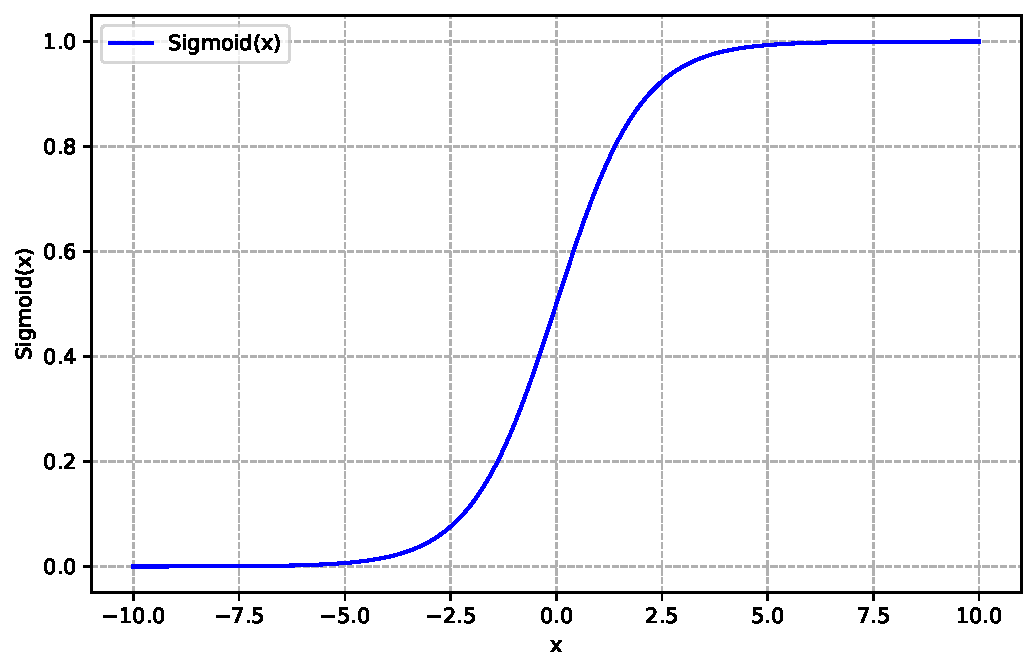
\includegraphics[width=1\linewidth]{Imagenes/03/Sigmoide.pdf}
    \captionof{figure}{Función sigmoide.}
\end{minipage}

\subsection{Capa \textit{Softmax}}

Las capas \textit{Softmax} (\textit{Softmax layers}) se usa típicamente como una capa de salida para tareas de multi-clasificación junto con la función error Entropía Cruzada. Su función es normalizar las salidas de las capas anteriores de tal modo que todas sumen uno. Normalmente, las unidades de capas anteriores nos darán un valor no normalizado acerca de como el valor de entrada se relaciona o depende con determinada clásica. La capa softmax normalizada lo que hace es, efectivamente, dar el valor de probabilidad de cada clase. 



\subsection{ReLU} 
\begin{minipage}{0.45\linewidth} 

La \textit{Rectified Linear Unit} (Unidad Lineal Rectificada) usada junto con la función de transformación lineal, usa la siguiente función de activación

\begin{equation}
    f(x) = \max (0,\omega x + b),
\end{equation}
Es usada en general como capa oculta. Se puede probar que las unidades ReLU dan gradientes muy consistentes, lo que mejora los métodos basados en estos.

\end{minipage} \hfill
\begin{minipage}{0.52\linewidth}
    \centering
    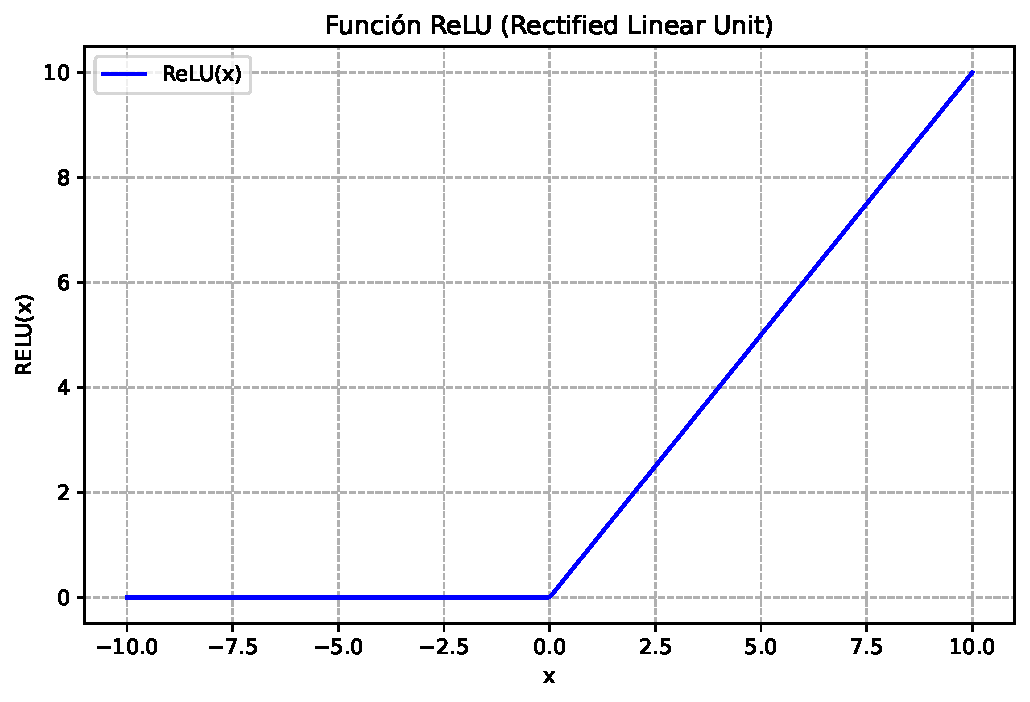
\includegraphics[width=1\linewidth]{Imagenes/03/ReLU.pdf}
    \captionof{figure}{Función sigmoide.}
\end{minipage}


\subsection{Tangente Hiperbólica}

\begin{minipage}{0.45\linewidth} 

    La tangente hiperbólica trnaforma el \textit{input} tal y como sigue: 

    \begin{equation}
        y = \tanh (\omega x + b)
    \end{equation}
    siendo claramente la función de activacióin

    \begin{equation}
        f(x) = \tanh (x)
    \end{equation}
    Se suele unidad como capa/unidad oculta, y en conjunción con la función de transoformación lineal. 

\end{minipage} \hfill
\begin{minipage}{0.52\linewidth}
    \centering
    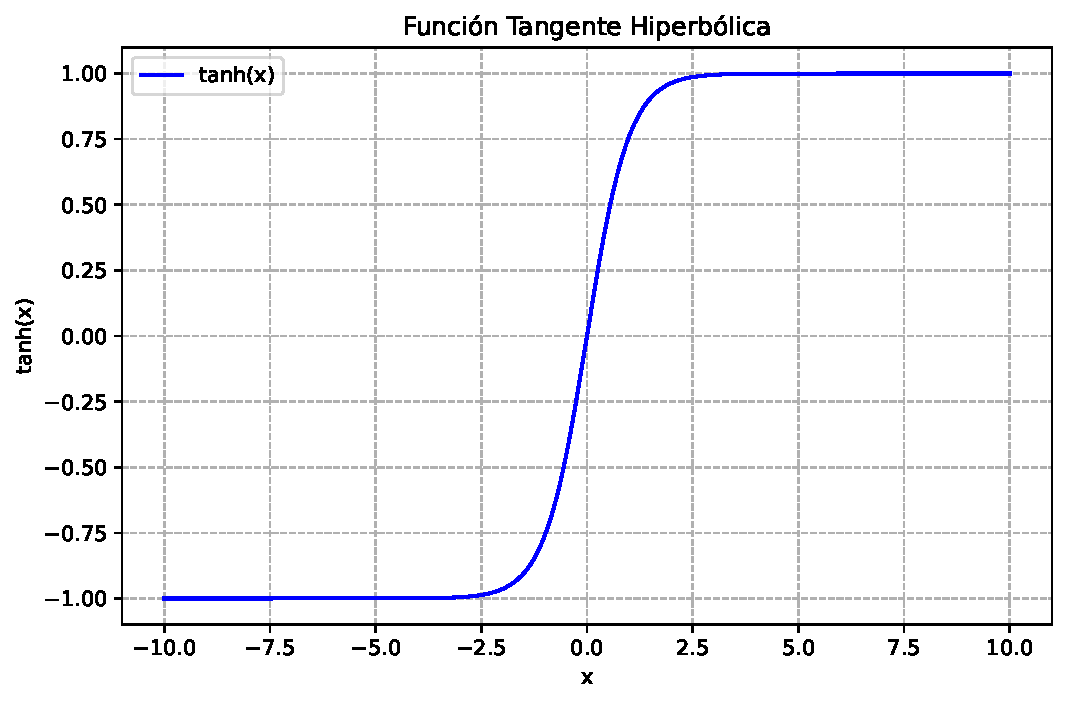
\includegraphics[width=1\linewidth]{Imagenes/03/Tanh.pdf}
    \captionof{figure}{Función sigmoide.}
\end{minipage}



\chapter{Redes Neuronales Convolucionales}

Las redes neuronales convolucionales o CNN (\textit{Convolutional Neural Network}) son, en esencia, redes neuronales que emplen métodos convolucionales en vez de usar capas completamente conectadas. Las CNNs son increíblemente exitosas en su aplicación a problemas en los que los datos de entrada sobre los que se van a realizar predicciones tienen una topología conocida en forma de malla, como una serie temporal (que es una malla unidimensional) o una imagen (que es una malla bidimensional).

\section{Operacion Convolucional}

La operación convolucional en una dimensión consta de dos partes, un \textit{input} $I(t)$ y un \textit{kernel} $K(a)$, tal que la \textbf{operación convolucional} es 

\begin{equation}
    s(t) = \sum_a I(a) \cdot K(t-a)
\end{equation}
Una forma equivalente 
\begin{equation}
    s(t) = \sum_a I(t-a) \cdot K(a)
\end{equation}
En la literatura del aprendizaje máquina y su implementación en \textit{software}, la convolución y la correlación cruzada son intercambiables. La esencia de la operación es qeu el Kernel, mucho más pequeño que el input. El valor de la convolción $s(t)$ será, como tal, la salida de la operación convolucion. Evidentemente podemos generalizar este resultado para \textit{inputs} y \textit{kernels} de varias dimensiones, tales como

\begin{equation}
    s(m,n) = (I * K) (m,n) = \sum_{a} \sum_{b} I(a,b) \cdot K(m-a,n-b)
\end{equation}
Podemos pensar en la convolución como el producto de un vector/matriz pequeño sobre un área de un valor grande (input) centrado dando como resultado un único valor. Repetiremos este proceso sobre varias ``áreas'' del input obteniendo un output vector/matriz. 

En las imagenes \cref{Fig:04-CNN_Convolucional} y \cref{Fig:04-CNN_LayerDensity} podemos ver dos diferentes tipos de redes neuronales. En este caso es evidente ver que, para el mismo número de entradas y salidas, la densamente conectada tiene muchas mas conexiones (y por tanto más pesos) que la red convolucional. Debido a esto, lógicamente las interacciones que producen las salidas serán menores, o que llamamos red de interacción escasa o dispersa (\textit{sparse interaction}). Dado que los parámetros y pesos se comparten a lo largo de la capa convolucional, ya que se usa siempre el mismo kernel en la interacción de una capa a otra, pues tendremos muchos menos parámetros que en una red no convolucional. 

\begin{minipage}{0.45\linewidth} \centering
\begin{tikzpicture}

% Capa inferior
\node[circle, draw, minimum size=10mm] (I1) at (0,0) {};
\node[circle, draw, minimum size=10mm] (I2) at (2,0) {};
\node[circle, draw, minimum size=10mm] (I3) at (4,0) {};
\node[circle, draw, minimum size=10mm] (I4) at (6,0) {};

% Capa superior
\node[circle, draw, minimum size=10mm] (O1) at (0,2) {};
\node[circle, draw, minimum size=10mm, ultra thick, red] (O2) at (2,2) {};
\node[circle, draw, minimum size=10mm] (O3) at (4,2) {};
\node[circle, draw, minimum size=10mm] (O4) at (6,2) {};

% Conexiones negras
\draw[arrows={->}] (I1) -- (O1);
\draw[arrows={->}] (I2) -- (O1);
\draw[arrows={->}] (I2) -- (O3);
\draw[arrows={->}] (I3) -- (O3);
\draw[arrows={->}] (I3) -- (O4);
\draw[arrows={->}] (I4) -- (O3);
\draw[arrows={->}] (I4) -- (O4);

% Conexiones rojas hacia O2
\draw[arrows={->}, red, thick] (I1) -- (O2);
\draw[arrows={->}, red, thick] (I2) -- (O2);
\draw[arrows={->}, red, thick] (I3) -- (O2);

\end{tikzpicture}
\captionof{figure}{Red Neuronal Convolucional}
\label{Fig:04-CNN_Convolucional}
\end{minipage} \hfill
\begin{minipage}{0.45\linewidth} \centering
\begin{tikzpicture}

% Capa inferior
\node[circle, draw, minimum size=10mm] (I1) at (0,0) {};
\node[circle, draw, minimum size=10mm] (I2) at (2,0) {};
\node[circle, draw, minimum size=10mm] (I3) at (4,0) {};
\node[circle, draw, minimum size=10mm] (I4) at (6,0) {};

% Capa superior
\node[circle, draw, minimum size=10mm] (O1) at (0,2) {};
\node[circle, draw, minimum size=10mm, ultra thick, red] (O2) at (2,3) {};
\node[circle, draw, minimum size=10mm] (O3) at (4,3) {};
\node[circle, draw, minimum size=10mm] (O4) at (6,2) {};

% Conexiones negras
\draw[arrows={->}] (I1) -- (O1);
\draw[arrows={->}] (I1) -- (O3);
\draw[arrows={->}] (I1) -- (O4);

\draw[arrows={->}] (I2) -- (O1);
\draw[arrows={->}] (I2) -- (O3);
\draw[arrows={->}] (I2) -- (O4);

\draw[arrows={->}] (I3) -- (O1);
\draw[arrows={->}] (I3) -- (O3);
\draw[arrows={->}] (I3) -- (O4);

\draw[arrows={->}] (I4) -- (O1);
\draw[arrows={->}] (I4) -- (O3);
\draw[arrows={->}] (I4) -- (O4);

% Conexiones rojas hacia O2
\draw[arrows={->}, red, thick] (I1) -- (O2);
\draw[arrows={->}, red, thick] (I2) -- (O2);
\draw[arrows={->}, red, thick] (I3) -- (O2);
\draw[arrows={->}, red, thick] (I4) -- (O2);

\end{tikzpicture}
\captionof{figure}{Red Neuronal con capas densamente conmunicadas.}
\label{Fig:04-CNN_LayerDensity}
\end{minipage}

\section{Operacion de Agrupamiento}

\begin{minipage}{0.5\linewidth}
La \textbf{operación de Agrupamiento} o \textit{pooling operation} es una técnica que se usa junto con la convolución en las CNN. La idea detrás de la operación de \textit{pooling} es que la ubicación exacta de la característica no es un problema si, de hecho, esta ha sido detectada. Simplemente proporciona invariancia ante traslaciones. Por ejemplo, supongamos que la tarea en cuestión es aprender a detectar rostros en fotografías. Supongamos también que los rostros en la fotografía están inclinados (como generalmente ocurre) y que tenemos una capa de convolución que detecta los ojos. Nos gustaría abstraer la ubicación de los ojos en la fotografía de su orientación. La operación de pooling logra esto y es un componente importante de las CNN.

\vspace*{0.6em}

Lo que hacen estas operaciones es coger porciones de los \textit{inputs} y aplicarles la función $f$, produciendo una salida. Esta función $f$, normalmente una operación $\max$ (puede haber otras), actúa sobre porciones regulares (al menos en 2 dimensiones) 
\end{minipage} \hfill
\begin{minipage}{0.45\linewidth}
    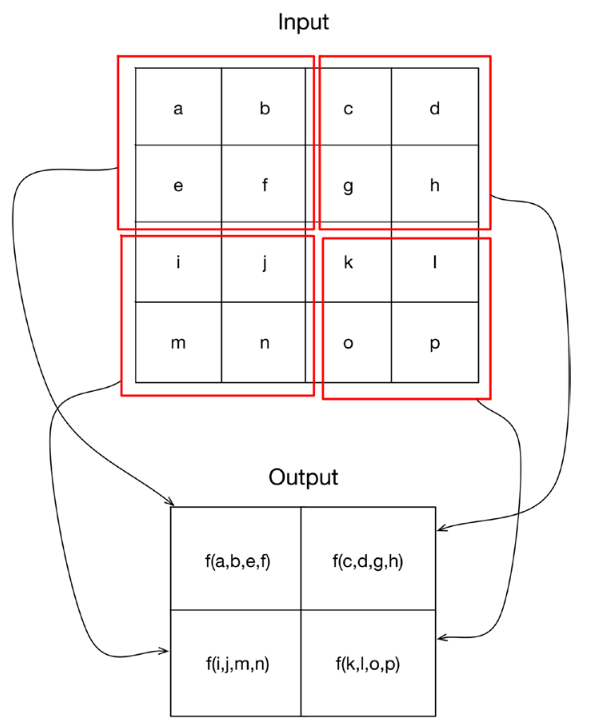
\includegraphics[width=1\linewidth]{Imagenes/04/Pooling.png}  
    \captionof{figure}{Ejemplo de una operación de Agrupamiento.} 
    \label{Fig:04-pooling}
\end{minipage}


y produce como resultado una salida dimensionalmente mucho más pequeña. En la \cref{Fig:04-pooling} representamos esta idea gráficamente. 

\section{Bloque básico de Convolución-Detector-Pooling}



\begin{minipage}{0.5\linewidth}
    
Ahora veremos como es un bloque básico en una red neuronal convolucional, donde mezclamos tanto procesos convolucionales como operaciones de agrupamiento. En la imagen \cref{Fig:04-pooling} vemos como una serie de inputs pasan a través de una red convolucional llegando pues a una capa o zona llamada detector (\textit{detector stage}) que es básicamente una función de activación no-lineal. La salida normalmente se pasa a otras capas (convolucionales o densamente conectadas). Lógicamente se pueden aplicar múltiples bloques de Convolución-Detector-Pooling en paralelo, utilizando la misma entrada y produciendo múltiples salidas o mapas de características (feature maps).

\end{minipage} \hfill
\begin{minipage}{0.45\linewidth}
    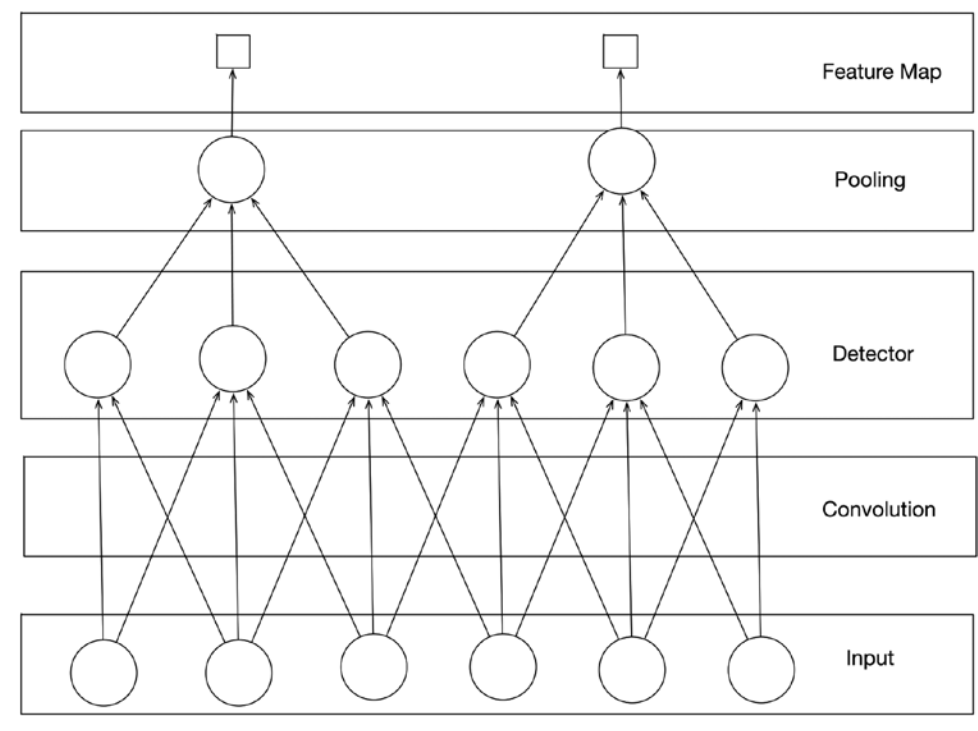
\includegraphics[width=1\linewidth]{Imagenes/04/PoolingBlock.png}  
    \captionof{figure}{Ejemplo de una operación de un bloque básico de detector-convolución-pooling.} 
    \label{Fig:04-poolingBlock}
\end{minipage}

\begin{minipage}{0.45\linewidth}
    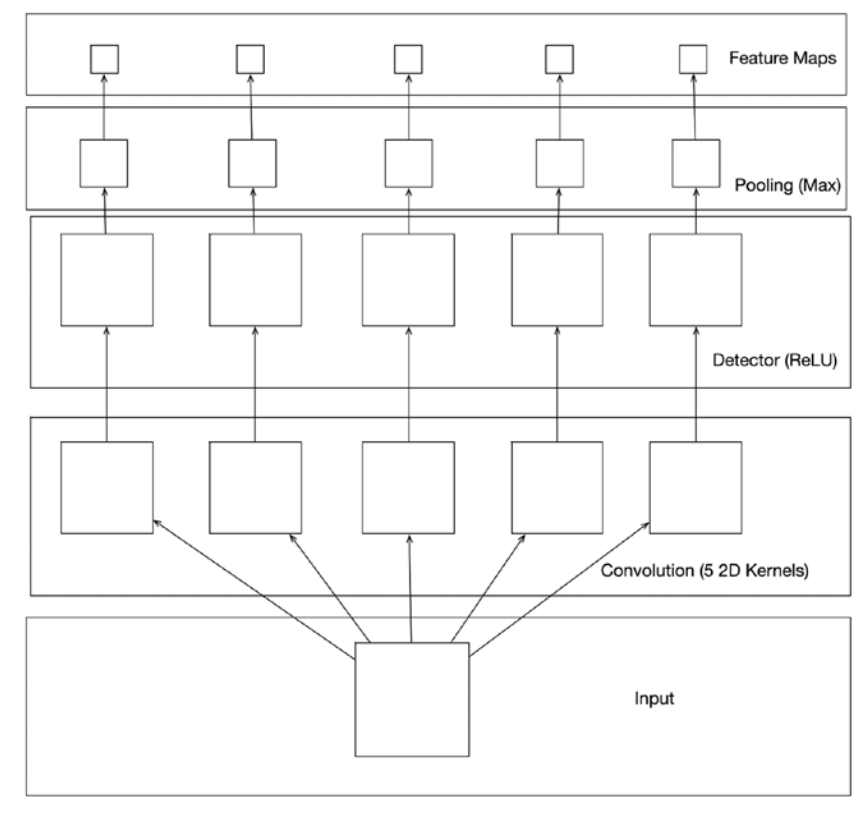
\includegraphics[width=1\linewidth]{Imagenes/04/PoolingFilter.png}  
    \captionof{figure}{Ejemplo de Kernels dando varias salidas.} 
    \label{Fig:04-poolingFilter}

\end{minipage} \hfill
\begin{minipage}{0.45\linewidth}
    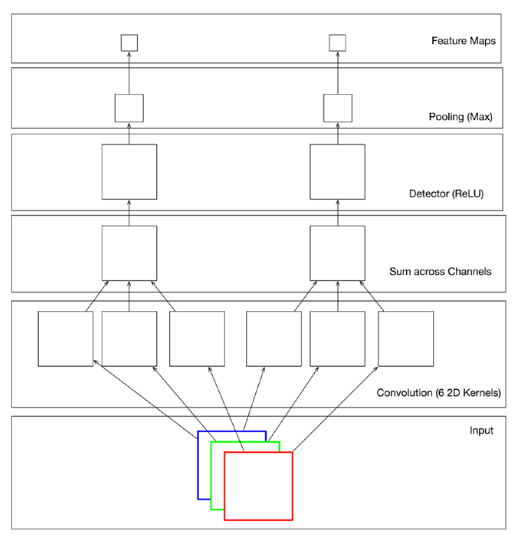
\includegraphics[width=1\linewidth]{Imagenes/04/PoolingMultiple.png}  
    \captionof{figure}{Convolución con varios canales.} 
    \label{Fig:04-poolingMultiple }
\end{minipage}

\section{Idea detrás de las redes neuronales convolucionales}

A lo largo de este capítulo hemos visto los conceptos básicos de las redes neuronales convolucionales, centrándonos en la operación convolución, la operación de agrupamiento o \textit{pooling} y como estas interactuan dentro de una CNN. Ahora bien, ¿Por qué se usan las CNNs? la primera idea que tenemos que considerar es su eficiencia. Las CNN, que en principio vienen a remplazar al menos una de las \textit{fully connected network}, en realidad tienen una pacaidad menor que estas, pero que a su vez, al tener menos parámetros únicos, deberían ser mucho más fáciles de entrenar (o al menos eficientemente). Otro de los aspectos a considerar vienen dados opr que, en realidad, los filtros manejados por la convolución, son capaces de detectar bordes, formas... Luego además debemos pensar en la operación agrupamiento, ya que esta en realidad nos permite separar el hecho de ser detectada una característica de la ubicación exacta de la característica (borde, forma...). Un filtro que detecta líneas rectas puede detectar este patrón en cualquier parte de la imagen, pero la operación de \textit{pooling} conserva el hecho de que la característica fue detectada (max \textit{pooling}). El útimo motivo es que la serie de capas de convolución y \textit{pooling} genera las características, y una red neuronal estándar aprende la función final de clasificación o regresión. Es importante distinguir este aspecto de las CNN del aprendizaje automático tradicional. En el aprendizaje automático tradicional, un experto diseñaba manualmente las características y las introducía en una red neuronal. En el caso de las CNN, estas características o representaciones se aprenden directamente a partir de los datos.
 \chapter{Redes Recurrentes}

 Las redes neuronales recurrentes son, en esencia, es un tipo de red que contiene conexiones recurrentes, es decir, conexiones en las que la salida de una neurona en un instante se utiliza como entrada para otra neurona en el instante siguiente. Esto permite a las RNNs capturar dependencias temporales y patrones secuenciales. 

\NewPart{Librerías de Python}{0.3}

\chapter{Theano}
\chapter{Keras}
\chapter{PyTorch}
\chapter{Tensor Flow}






\end{document}